\documentclass[11pt,spanish]{article}

% Paquetes
\usepackage{amstext}
\usepackage{amssymb}
\usepackage{babel}
    \addto\shorthandsspanish{\spanishdeactivate{~<>}}
    \decimalpoint
\usepackage[style=iso]{datetime2}
\usepackage{fancyhdr}
\usepackage{float}
\usepackage[T1]{fontenc}
\usepackage[a4paper]{geometry}
    \geometry{verbose,tmargin=3cm,bmargin=2cm,lmargin=2cm,rmargin=2cm}
\usepackage{graphicx}
\usepackage[utf8]{inputenc}
\usepackage{lastpage}
\usepackage{mathptmx}
\usepackage{units}

% tipo de fuente 
\usepackage{lmodern}

\pagestyle{fancy}
\lfoot{\small DF, FCEyN, UBA}
\cfoot{\tiny Actualizado el {\today} a las {\DTMcurrenttime}}
\rfoot{\small Pág. {\thepage} de \pageref{LastPage}}

\begin{document}

% Título
    \begin{center}
    \textsc{\large Física 2 (Física) -- Cátedra Diego Arbó}
    \par\end{center}{\large \par}
    
    \begin{center}
    \textsc{\large Primer Cuatrimestre de 2025}
    \par\end{center}{\large \par}
    
    \begin{center}
    \textsc{\large Repaso: Números Complejos}
    \par\end{center}{\large \par}

% Comienzo 
\begin{enumerate}

% Ejercicio 1

    \item Para cada uno de los siguientes números, halle sus partes real e imaginaria,
    y dibújelos en el plano complejo:

    \begin{enumerate}
        \item $0$
        \item $\pm 1$
        \item $\pm i$
        \item $i^2$
        \item $0 i$
        \item $a$ (con $a$ real)
        \item $b i$ (con $b$ real)
        \item $1 \pm i$
        \item $-1 \pm i$
        \item $\cos(\theta) \pm i \sin(\theta)$ (con $\theta$ entre $0$ y $2 \pi$) 
        \item $a \pm bi$ 
        \item $\pm \sqrt {a^2 + b^2}$
        \item $\pm i \sqrt {a^2 + b^2}$
        \item $ (a + bi)^2 $
    \end{enumerate}

    \textbf{Nota:} $a$, $b$ y $\theta$ son números reales.

% Ejercicio 2

    \item Para un número complejo $z$, se define su módulo $|z|$ como la distancia euclídea que separa a $z$ del origen del plano complejo. Escriba la expresión más general para el módulo de $z$ en función de sus partes real e imaginaria, y luego aplíquela a cada caso del primer ejercicio.

% Ejercicio 3

    \item Se define el argumento $\arg(z)$ de un número complejo $z$ como el ángulo $\theta$ formado entre el eje real y la línea que va desde el origen a $z$, considerando positivo al sentido de giro que va desde el eje $\mathfrak{Re}^+$ hacia el eje $\mathfrak{Im}^+$.

    \begin{figure}[H]
        \centering{}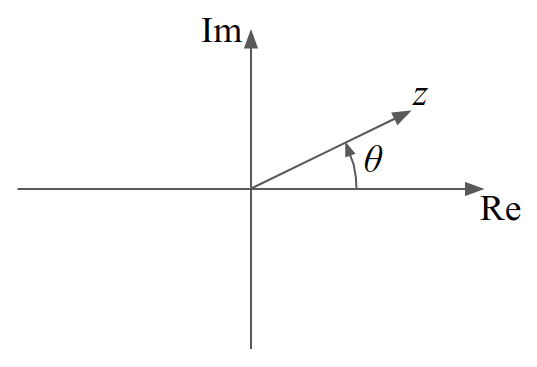
\includegraphics[clip,scale=0.35]{figs/ej0}
    \end{figure}

    Halle el argumento para todos los casos del primer ejercicio.
    
% Ejercicio 4

    \item Se define el conjugado de un número complejo $z = a + bi$ como $\overline{z} = a - bi$.
    \begin{enumerate}
        \item Verifique que el conjugado de un número real es ese mismo número real. 
        \item Verifique que el conjugado de un número imaginario puro es ese mismo número multiplicado por $-1$.
        \item Verifique que el conjugado de un número complejo arbitrario corresponde a una reflexión (en el plano complejo) del número original respecto al eje real.
        \item ¿Cuál es el conjugado de 0?
    \end{enumerate}

    \textbf{Nota:} El conjugado de $z$ suele representarse también como $z^*$.
% Ejercicio 5

    \item Obtenga el conjugado para todos los números del primer ejercicio, y determine sus partes real e imaginaria, su módulo y su argumento. Si es posible, use los resultados anteriores para ahorrar cuentas.

% Ejercicio 6

    \item Verifique la siguiente identidad:
    
        $$z\overline{z} = |z|^2$$

% Ejercicio 7

    \item Halle las partes real e imaginaria de los siguientes números:
    
    \begin{enumerate}
        \item $\frac{1+i}{1-i}$
        \item $\frac{1+i}{1+i}$
        \item $(1+i)(1-i)$
        \item $(1+i)^2$
        \item $(1+i)^3$
        \item $(1+i)^4$
        \item $\sqrt{(1+i)(1-i)}$
        \item $i^0$
        \item $i^n$ (con $n$ entero positivo)
        \item $\nicefrac{1}{i^n}$ (con $n$ entero positivo)
        \item $\nicefrac{1}{(a + bi)}$ (con $a$ y $b$ número reales, y $|a + bi|$ distinto de $0$)	
        \item $1 / (\cos(\theta) + i \sin(\theta))$
    \end{enumerate}
    
    \textbf{Ayuda:} Puede ser útil emplear la identidad del ejercicio anterior para trabajar con denominadores complejos.

% Ejercicio 8

    \item ¿Cuáles de los siguientes datos me permiten determinar completamente a un número complejo cualquiera?
    
    \begin{enumerate}
        \item Su parte real y su parte imaginaria
        \item Su parte real y la parte imaginaria de su conjugado
        \item Las partes real e imaginaria de su conjugado
        \item Su módulo y su parte real
        \item Su módulo y su parte imaginaria
        \item Su módulo y su argumento
        \item Su argumento y su parte real
        \item Su argumento y su parte imaginaria
    \end{enumerate}

% Ejercicio 9

    \item Compare el plano complejo con el plano $\mathbb{R}^2$. Analice similitudes y diferencias entre vectores de $\mathbb{R}^2$ y números complejos. ¿Es posible pensar a un número complejo como un vector? ¿Qué forma de representar un número complejo se parece a la representación cartesiana de un vector? ¿Y a la representación polar?

% Ejercicio 10

    \item Considere la fórmula de Euler:
    $$e^{ix} = \cos(x) + i \sin(x)$$
    A partir de la misma, demuestre la identidad de Euler:
    $$e^{i\pi} + 1 = 0$$
    
% Ejercicio 11

    \item Un número complejo z puede representarse en forma polar de la siguiente manera:

    $$z = |z|e^{i \arg(z)}$$

    \begin{enumerate}
        \item Obtenga las partes real e imaginaria a partir de dicha representación.
        
        \item Verifique, a partir de la definición de complejo conjugado, que el conjugado de $e^{i \theta}$ es $e^{-i \theta}$.
    \end{enumerate}
    

% Ejercicio 12

    \item Obtenga y grafique las partes real e imaginaria de las siguientes funciones del tiempo:

    \begin{enumerate}
        \item $\exp(i \omega t)$
        \item $\exp(-i \omega t)$
        \item $\exp(i (\omega t + \pi/2))$
        \item $\exp(i (\omega t - \pi/2))$
        \item $\exp(i \omega_1 t) + \exp(i \omega_2 t) $
        \item $i \exp(i \omega t)$
        \item $-\exp(i \omega t)$
        \item $\nicefrac{1}{2} (\exp(i \omega t) + \exp(-i \omega t))$
        \item $\nicefrac{1}{(2i)} (\exp(i \omega t) - \exp(-i \omega t))$
    \end{enumerate}

% Ejercicio 13

    \item A partir de la fórmula de Euler, demuestre que:
    
    \begin{enumerate}
        \item $\cos(x) = \nicefrac{1}{2}(e^{ix} + e^{-ix})$
        \item $\sin(x) = (e^{ix} - e^{-ix}) / (2i)$
        \item $\cosh(x) = \cos(ix)$ (con $x$ real)
        \item $\sinh(x) = -i \sin(ix)$ (con $x$ real)
    \end{enumerate}
    
% Ejercicio 14

    \item Verifique la identidad trigonométrica del coseno de la suma y resta de ángulos mediante la fórmula de Euler. (\textbf{Ayuda:} desarrolle el lado derecho mediante exponenciales complejas; no hace falta tomar parte real.) ¿Cómo puede obtener la identidad correspondiente al seno?

% Ejercicio 15

    \item Use la fórmula de Euler para hallar las dos raices cuadrada de i, escritas mediante sus partes real e imaginaria.

\end{enumerate}

\end{document}
